\documentclass[aspectratio=169]{beamer}

% Essential packages
\usepackage[utf8]{inputenc}
\usepackage[T1]{fontenc}
\usepackage[english]{babel}
\usepackage{graphicx}
\usepackage{tikz}
\usepackage{array}
\usepackage{ragged2e}

\newcolumntype{L}[1]{>{\RaggedRight\arraybackslash}p{#1}}

% Modern Roboto font
\usepackage[sfdefault]{roboto}
\usepackage[T1]{fontenc}

% Color definitions
\definecolor{vermelhoPrincipal}{HTML}{b11116}
\definecolor{azulComplementar}{HTML}{3a5461}
\definecolor{brancoFundo}{HTML}{FFFFFF}

% Theme configuration
\usetheme{Madrid}
\usecolortheme{default}

% Custom colors - text always black
\setbeamercolor{structure}{fg=black}
\setbeamercolor{palette primary}{bg=vermelhoPrincipal,fg=white}
\setbeamercolor{palette secondary}{bg=azulComplementar,fg=white}
\setbeamercolor{palette tertiary}{bg=vermelhoPrincipal,fg=white}
\setbeamercolor{palette quaternary}{bg=azulComplementar,fg=white}
\setbeamercolor{frametitle}{bg=vermelhoPrincipal,fg=white}
\setbeamercolor{background canvas}{bg=brancoFundo}
\setbeamercolor{title}{fg=black}
\setbeamercolor{subtitle}{fg=azulComplementar}
\setbeamercolor{author}{fg=black}
\setbeamercolor{date}{fg=black}
\setbeamercolor{itemize item}{fg=black}
\setbeamercolor{itemize subitem}{fg=black}
\setbeamercolor{enumerate item}{fg=black}
\setbeamercolor{block title}{bg=vermelhoPrincipal,fg=white}
\setbeamercolor{block body}{bg=vermelhoPrincipal!10,fg=black}
\setbeamercolor{normal text}{fg=black}

% Itemize font configuration
\setbeamerfont{itemize/enumerate body}{size=\scriptsize}
\setbeamerfont{itemize/enumerate subbody}{size=\scriptsize}

% Modern, minimalist bullets
\setbeamertemplate{itemize item}{\raisebox{0.2ex}{\rule{0.6ex}{0.6ex}}}
\setbeamertemplate{itemize subitem}{\raisebox{0.3ex}{\rule{0.4ex}{0.4ex}}}
\setbeamertemplate{itemize subsubitem}{\raisebox{0.35ex}{\rule{0.3ex}{0.3ex}}}
\setbeamertemplate{enumerate items}[square]

% Smooth transitions
\setbeamercovered{transparent}

% Remove navigation symbols
\setbeamertemplate{navigation symbols}{}

% Custom header with red bar and logos
\setbeamertemplate{headline}{
  \begin{beamercolorbox}[wd=\paperwidth,ht=0.6cm,dp=0.15cm,leftskip=0.2cm,rightskip=0.4cm]{palette primary}
    \raisebox{-0.05cm}{\includegraphics[height=0.45cm]{imgs/base/fatec-rgt.png}}
    \hfill
    \raisebox{-0.18cm}{\includegraphics[height=0.85cm]{imgs/base/governo-sp-secretaria-logo.png}}
    \hspace{0.2cm}
    \raisebox{-0.08cm}{\includegraphics[height=0.6cm]{imgs/base/cps-logo.png}}
  \end{beamercolorbox}
}
% Remove block shadows
\setbeamertemplate{blocks}[default]
\setbeamertemplate{itemize/enumerate body begin}{\scriptsize}
\setbeamertemplate{itemize/enumerate subbody begin}{\scriptsize}
% Custom footer
\setbeamertemplate{footline}{
  \begin{beamercolorbox}[wd=\paperwidth,ht=0.4cm,dp=0.2cm,leftskip=0.3cm,rightskip=0.3cm]{palette secondary}
    \usebeamerfont{footline}
    \insertshortauthor \hfill \hfill {\fontsize{5}{6}\selectfont\insertshorttitle} \hfill \hfill \insertframenumber/\inserttotalframenumber
  \end{beamercolorbox}
}

% Custom frame title
\setbeamertemplate{frametitle}{
  \vspace{0.3cm}
  \textcolor{black}{\insertframetitle}
  \vspace{0.1cm}
}

% Presentation information
\title{Shrimp Farming with IoT \\Monitoring for the Culinary Sector}
\subtitle{}
\author[DSM]{ALMEIDA, D.; MUNIZ, L.; RODRIGUES, T.}
\institute{Multiplatform Software Development\\FATEC Registro}
\date{\today}

\begin{document}

% Modern title slide
\begin{frame}
  \vspace{0.8cm}
  \begin{center}
    
\begin{tikzpicture}
      % Top decorative line
      \draw[vermelhoPrincipal, line width=2pt] (-4,0) -- (4,0);
    \end{tikzpicture}
    
    \vspace{0.4cm}
    
    {\normalsize\bfseries\inserttitle}\par
    
    \vspace{0.2cm}
    
    {\tiny\insertauthor}\par
    
    \vspace{0.1cm}
    
    {\small\textcolor{azulComplementar}{\insertsubtitle}}\par
    
    \vspace{0.5cm}
    
    
\begin{tikzpicture}
      % Bottom decorative line
      \draw[azulComplementar, line width=1.5pt] (-2.5,0) -- (2.5,0);
    \end{tikzpicture}
    
    \vspace{0.3cm}
    
    {\scriptsize\insertinstitute}\par
    
    \vspace{0.01cm}
    
    {\tiny\textcolor{azulComplementar}{\insertdate}}\par
  \end{center}
\end{frame}

\section{Agenda}
{
\usebackgroundtemplate{%
  \includegraphics[width=\paperwidth,height=\paperheight]{imgs/teste.png}%
}

% Agenda slide
\begin{frame}[b]{Agenda}
  \begin{itemize}
    \item Pitch
    \item Problem Statement
    \item State of the Art
    \item Objective
    \item Tools and Technologies
    \item Methodology
    \item Practical Demonstration
    \item Results and Discussion
  \end{itemize}
  
  \vfill
  
  \hfill{\scriptsize \textbf{Duration:} 10 to 11 min.}
\end{frame}

\section{Pitch}
{
\usebackgroundtemplate{%
  \includegraphics[width=\paperwidth,height=\paperheight]{imgs/LOGO.png}%
}
\begin{frame}[b]{Pitch}

\end{frame}
}

\section{Problem Statement}

{
\usebackgroundtemplate{%
  \includegraphics[width=\paperwidth,height=\paperheight]{imgs/teste.png}%
}
\begin{frame}[b]{Problem Statement}
  \begin{itemize}
    \item \parbox{0.60\textwidth}{Predominantly manual management}
    \item \parbox{0.60\textwidth}{Lack of automated control}
    \item \parbox{0.60\textwidth}{No historical record of environmental parameters}
  \end{itemize}
  
  \vfill
  
  {\fontsize{4}{5}\selectfont\textit{Source: Your Name}\hfill\textcolor{white}{Image: Image description}}
\end{frame}
}

\section{State of the Art}

{
\usebackgroundtemplate{}
\begin{frame}[t]{State of the Art}

\begin{table}
    \centering
    \tiny
    \begin{tabular}{|L{2.5cm}|L{2cm}|L{2cm}|L{2cm}|L{2cm}|L{1.5cm}|}
      \hline
      \textbf{Title/Authors} & \textbf{Objective} & \textbf{Method} & \textbf{Results} & \textbf{Limitations} & \textbf{Gap} \\
      \hline
      Telemonitoring system for shrimp farming — Dantas (2020) & Monitor temperature, pH and dissolved oxygen in shrimp ponds & ESP32 with LoRaWAN and AWS integration via MQTT & 0.5°C temperature variation and 138-meter range & No ammonia monitoring and low energy autonomy & No feeding control and no historical logging \\
      \hline
      Real-time monitoring for freshwater shrimp farms — Uddin (2020) & Monitor water quality and survival rate in a real farming setting & Arduino Yun with multiple sensors, cloud-based AHP method and web notifications & 4,600+ records, error below 7\%, 90\% survival & Exclusive reliance on Wi-Fi and need for frequent manual calibration & No feeding automation and no ammonia monitoring \\
      \hline
      IoT-based Vaname shrimp water quality monitoring prototype using Google Spreadsheet — Wisaksono (2024) & Monitor water quality in Vannamei shrimp farming (temperature, pH and conductivity/TDS) with remote access via smartphone & Arduino Uno coupled to NodeMCU ESP8266 via serial port, with DS18B20, PH SEN0161 and TDS sensors; data sent over Wi-Fi to Google Sheets & Accuracy of 98.59\% (TDS), 98.59\% (DS18B20) and 94.89\% (pH), with standard deviations of 0.448, 0.053 and 0.258 & Results depend on specific environmental conditions and sensor calibration, limiting generalization; no dissolved oxygen or ammonia monitoring & No feeding control and no preventive alerts \\
      \hline
    \end{tabular}
  \end{table}
\end{frame}
}

\section{Objective}

{
\usebackgroundtemplate{%
  \includegraphics[width=\paperwidth,height=\paperheight]{imgs/teste.png}%
}
\begin{frame}[b]{Objective}
  \begin{itemize}
    \item \parbox{0.60\textwidth}{\textbf{General objective}: Develop an automated monitoring system for shrimp farming tanks.}
    \item \parbox{0.60\textwidth}{\textbf{Specific objectives}:}
    \begin{itemize}
      \item \parbox{0.55\textwidth}{Remotely monitor environmental parameters (temperature, pH, ammonia)}
      \item \parbox{0.55\textwidth}{Record and store historical data from the tanks}
      \item \parbox{0.55\textwidth}{Automate feed delivery}
      \item \parbox{0.60\textwidth}{Provide a responsive web application}
    \end{itemize}
  \end{itemize}
  
  \vfill
  
  {\fontsize{4}{5}\selectfont\textit{Source: Your Name}\hfill\textcolor{white}{Image: Image description}}
\end{frame}
}

\section{Tools and Technologies}

{
\usebackgroundtemplate{%
  \includegraphics[width=\paperwidth,height=\paperheight]{imgs/teste.png}%
}
\begin{frame}[b]{Tools and Technologies}
  \begin{itemize}
  \item \parbox{0.60\textwidth}{\textbf{Languages}: JavaScript, TypeScript, Arduino/C++}
  \item \parbox{0.60\textwidth}{\textbf{Frameworks}: Express.js, Next.js 14, React 18, Mongoose}
  \item \parbox{0.60\textwidth}{\textbf{Database}: MongoDB Atlas (cloud)}
  \item \parbox{0.60\textwidth}{\textbf{Infrastructure}: Docker, Node.js 18+, Alpine Linux}
  \item \parbox{0.60\textwidth}{\textbf{Tools}: Git, Vercel, Render, Swagger/OpenAPI 3.0}
  \item \parbox{0.60\textwidth}{\textbf{APIs and integrations used}: Nodemailer, MongoDB Atlas API, NTP Server, Web Push API, JWT, Axios, DallasTemperature, OneWire, HTTPClient}
  \end{itemize}
  
  \vfill
  
  {\fontsize{4}{5}\selectfont\textit{Source: Your Name}\hfill\textcolor{white}{Image: Image description}}
\end{frame}
}

\section{Methodology}

{
\usebackgroundtemplate{}
\begin{frame}[t]{Methodology}
  \centering
  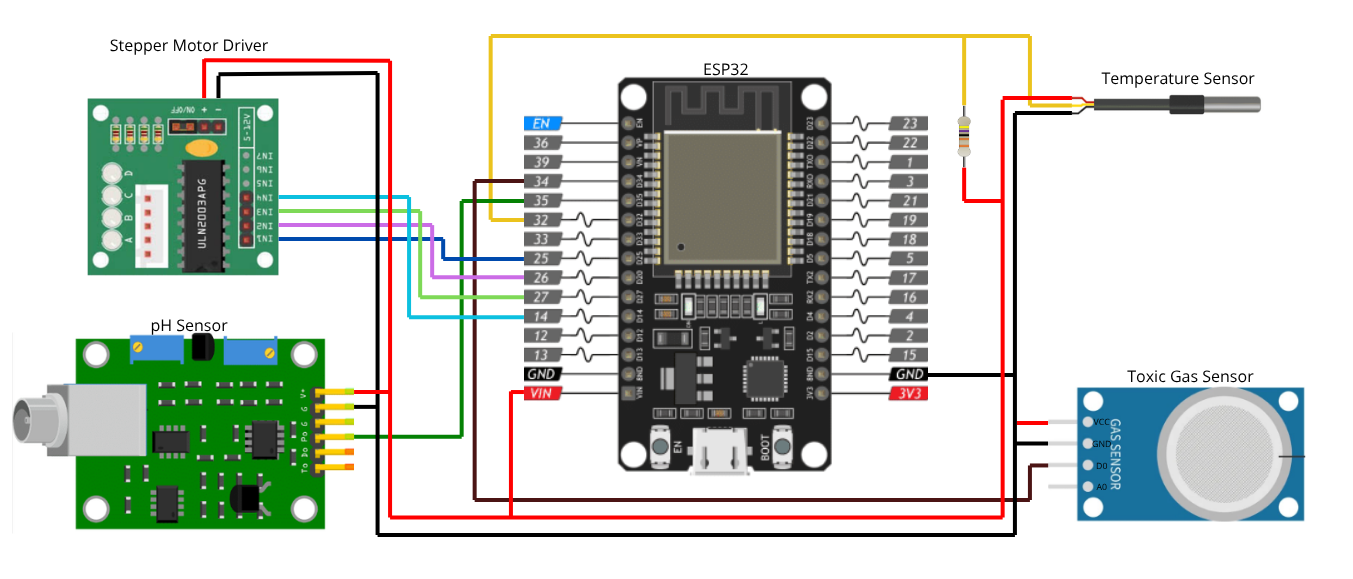
\includegraphics[width=0.8\paperwidth,keepaspectratio]{imgs/diagrama-iot-camarize-ingles.png}
\end{frame}
}

{
\usebackgroundtemplate{}
\begin{frame}[t]{Methodology}
  \centering
  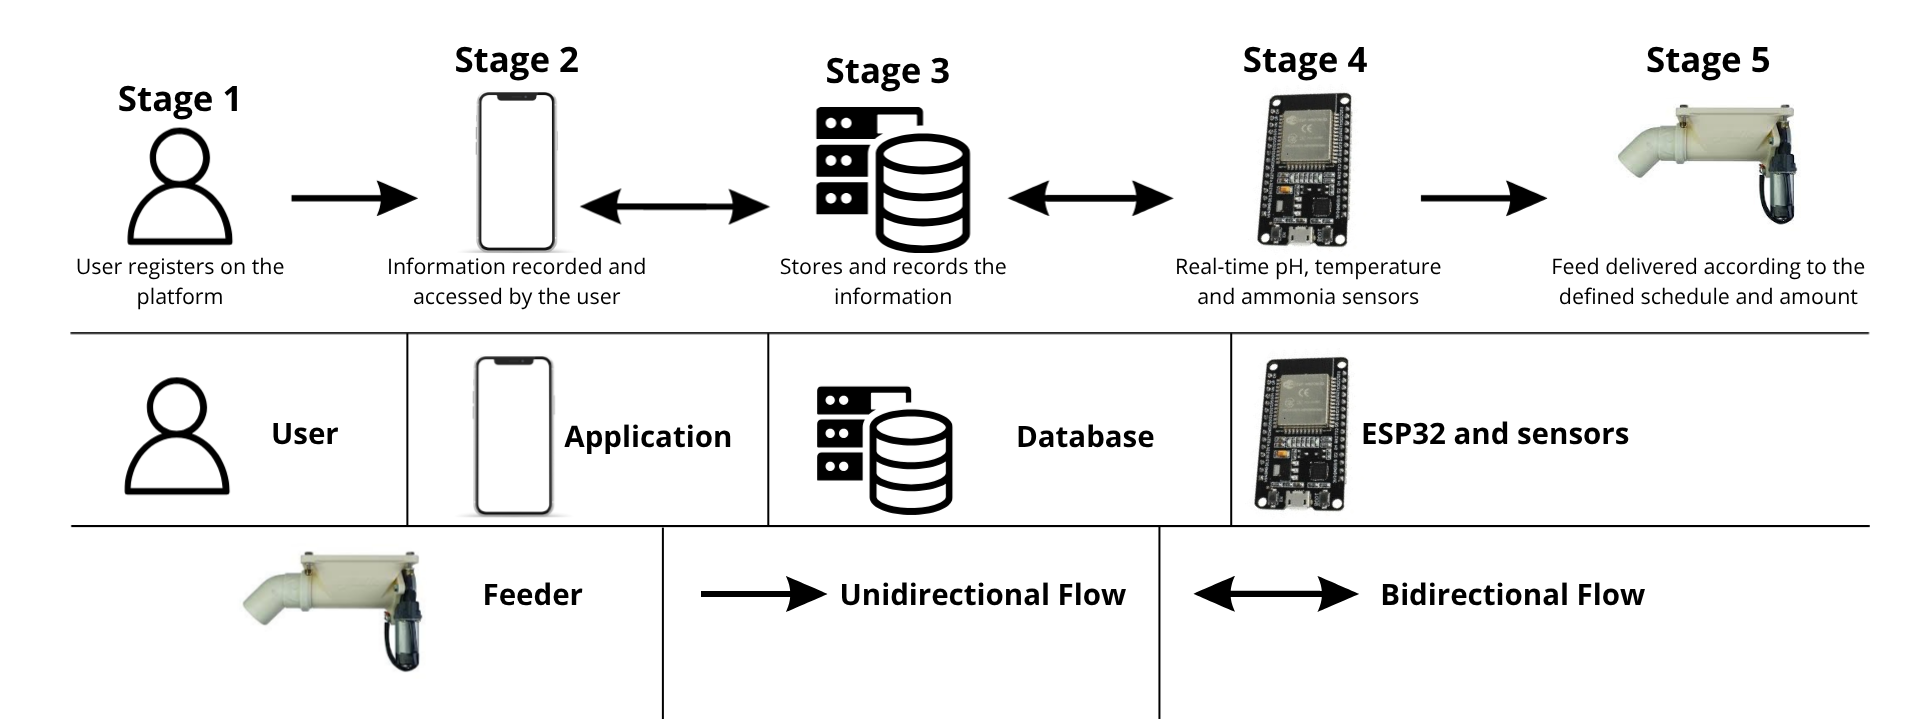
\includegraphics[width=0.8\paperwidth,keepaspectratio]{imgs/fluxograma-camarize-ingles.png}
\end{frame}
}

\section{Practical Demonstration}

{
\usebackgroundtemplate{%
  \includegraphics[width=\paperwidth,height=\paperheight]{imgs/LOGO.png}%
}
\begin{frame}[b]{Practical Demonstration}
  
  \vfill
  
  {\fontsize{4}{5}\selectfont\textit{Source: Own authorship}\hfill\textcolor{white}{Image: Image description}}
\end{frame}
}

\section{Results and Discussion}

{
\usebackgroundtemplate{}
\begin{frame}[t]{Results and Discussion}
  \begin{table}[H]
    \centering
    \resizebox{\textwidth}{!}{%
    \begin{tabular}{ccccccc}
      \hline
      \textbf{Test} & \textbf{Actual Temp. (°C)} & \textbf{Sensor Temp. (°C)} & \textbf{Actual pH} & \textbf{Sensor pH} & \textbf{Actual Ammonia} & \textbf{Sensor Ammonia} \\
      \hline
      1 & 21.0 & 20.50 & 7.0 & 6.79 & 0.000 & 0.000 \\
      2 & 26.0 & 25.79 & 7.0 & 6.79 & 0.000 & 0.000 \\
      3 & 17.0 & 16.80 & 7.0 & 6.79 & 0.000 & 0.000 \\
      4 & 21.0 & 20.50 & 5.0 & 4.80 & 0.000 & 0.000 \\
      5 & 22.0 & 21.60 & 8.6 & 7.90 & 0.000 & 0.000 \\
      6 & 22.0 & 21.60 & 7.0 & 6.79 & 0.000 & 0.000 \\
      \hline
      \textbf{Mean error} & \multicolumn{2}{c}{\textbf{1.73\%}} & \multicolumn{2}{c}{\textbf{4.02\%}} & \multicolumn{2}{c}{—} \\
      \textbf{Mean accuracy} & \multicolumn{2}{c}{\textbf{98.27\%}} & \multicolumn{2}{c}{\textbf{95.98\%}} & \multicolumn{2}{c}{—} \\
      \hline
    \end{tabular}}
    \label{tab:sensores}
  \end{table}
\end{frame}
}

{
\usebackgroundtemplate{%
  \includegraphics[width=\paperwidth,height=\paperheight]{imgs/teste.png}%
}
\begin{frame}[b]{Results and Discussion}
\begin{itemize}
  \item \parbox{0.60\textwidth}{Main \textbf{results} achieved: real-time monitoring, automatic alerts and remote feeding control}
  \item \parbox{0.60\textwidth}{\textbf{Metrics} analysis: 98.27\% accuracy (temperature) and 95.98\% (pH), alerts in 1 minute}
  \item \parbox{0.60\textwidth}{\textbf{User} feedback: 6 tests in a real environment, interface approved in usability}
  \item \parbox{0.60\textwidth}{\textbf{Challenges}: MQ-135 sensor limited in aquatic environments and mechanical instability in the dispenser}
  \item \parbox{0.60\textwidth}{Contributions and \textbf{lessons learned}: technical feasibility of a unified, low-cost IoT system}
  \item \parbox{0.60\textwidth}{\textbf{Future work}: submersible ion-selective sensor, dispenser redesign and validation in a commercial farm}
\end{itemize}
  
  \vfill
  
  {\fontsize{4}{5}\selectfont\textit{Source: Your Name}\hfill\textcolor{white}{Image: Image description}}
\end{frame}
}

% General information slide (clone)
{
\usebackgroundtemplate{%
  
\includegraphics[width=\paperwidth,height=\paperheight]{imgs/obrigado-ingles.png}%
}
\begin{frame}[b]{}
  \vspace{0.2cm}
  
  \hspace*{0.25\paperwidth}
  
  \vfill
\end{frame}
}

\end{document}